\documentclass{article}
\usepackage[utf8]{inputenc}
\usepackage{graphicx}
\graphicspath{ {diagrams/}  }

\title{NAVUP\\ Software Requirements Specification\\ University of Pretoria}
\author{Darren Adams\hspace{2 cm} - u14256232\\ Keanan Jones\hspace{2 cm} - u13036892\\ Lesego Makaleng\hspace{2 cm} - u15175716\\ Dedre Olwage\hspace{2 cm} - u15015239\\ Kamogelo Tsipa\hspace{2 cm} - u13010931 }
\date{February 2017}

\begin{document}

\maketitle
\pagebreak
\tableofcontents
\pagebreak
\section{Introduction}
    \subsection{Purpose}
		\begin{flushleft}
			This document serves the purpose of providing an intensive description for the NavUP system(product). It will also identify the possible requirements and restrictions for the NavUP system(product). This document will help the developer to gain insight on what the system(product) should do, to better understand how the system should be implemented in the implementation phase.
		\end{flushleft}
    \subsection{Scope}
		\begin{flushleft}
			The system(product) to be developed is called NavUP. NavUP will serve as a navigation application. NavUP intends to provide different users with optimal routes to destinations across the University of Pretoria campus.
			
			Furthermore NavUP provides a way saving and searching locations, both indoors and outdoors. NavUP will also facilitate search-ability of POIs and events. The Wi-Fi infrastructure within campus will be used for administering location and navigation services.
		\end{flushleft}
    \subsection{Definitions, Acronyms and Abbreviations}
        \begin{table}[h!]
            \centering
            \begin{tabular}{|c|c|}
            \hline
            Term & Definition \\
            \hline
            POI & Point of Interest \\
            \hline
            Wi-Fi & Wireless network infrastructure \\
            \hline
            Developer & Person/s developing the system. COS301 Software Engineers
            \\
            \hline
            GPS & Global Positioning System used by devices to determine current locations
            \\
            \hline
            Heat Maps & Graphical representation of data in the form of colours on a map.
            \\
				  \hline
            UC & Use Case
            \\
 				\hline
            TUCBW & This Use Case Begins With
            \\
			   \hline
            TUCEW & This Use Case Ends With
            \\
 				\hline
            TUCCW & This Use Case Continues With
            \\
				 \hline
            ETA & Estimated Time of Arrival
            \\
            \hline
            \end{tabular}
        \end{table}
    \subsection{Overview}
		\begin{flushleft}
			In this document, an Overall Description will be provided for the NavUP system(product). In the Overall Description, the Product Perspective, Product Functions, User Characteristics and Constraints will be discussed. Following the Overall Description, will be an elaboration on the Specific Requirements for the NavUP system(product). For the Specific Requirements, External Interface Requirements, Functional Requirements, Performance Requirements, Design Constrants, Software Sytem Attributes and Other Requirements will be identified and discussed.
Thereafter, any relevant appendixes and indexes needed by this document will be provided.
		\end{flushleft}
\section{Overall Description}

    \begin{flushleft}
        This section provides an overview of the system as a whole. We will explain how the system works, as well as how it interacts with other systems.
    \end{flushleft}
    
    
    \subsection{Product Perspective}
    
        NavUP is a mobile application used by students at the University of Pretoria. NavUP provides navigation of campus, providing traffic congestion and location services. NavUP will rely on other NavUP devices for real-time statistics and will interact with a primary server for pre-determined locations, events, POIs and venues. Both NavUP server and NavUP mobile will be present on the same network.
        \subsubsection{System Interfaces}
        Todo: Identifying interacting subsystems first needs to be done.
        \subsubsection{User Interfaces}
            Interaction between user and system will be achieved through the use of a GUI.        
        \subsubsection{Hardware Interfaces}
        \subsubsection{Software Interfaces}
        \subsubsection{Communication Interfaces}
        \subsubsection{Memory}
        \subsubsection{Operations}
        \subsubsection{Site Adaptation Requirements}
    \subsection{Product Functions}
		\begin{flushleft}
			General functions for the NavUP system(product) include:
			\begin{itemize}
   		 	\item The ability to use several Wi-Fi connection points as navigation tools
			 	\item The ability to calculate optimal routes from one destination to another, bases on the user's needs (i.e it must cater for routes for those with disabilities etc.).
			 	\item The ability to provide accurate information about pedestrain traffic based on how many devices are connected to certain Wi-Fi connection points.
				 \item The ability to reroute the user based on certain preferences.
				 \item The ability to calculate the user's current location while indoors and while outdoors.
				 \item The ability to search for locations, save locations, and providing directions to a location. 
			\end{itemize}
		\end{flushleft}
    \subsection{User Characteristics}
        \begin{flushleft}
            Students, Lecturers and Guests will interact with the system.
            \break
            Students will interact for venues used for classes for modules, social events and places of interest.
            Guests will interact for navigation to locations unknown to them.
            Lecturers will use the system for efficient traffic-free routing.
        \end{flushleft}
    \subsection{Constraints}
        \begin{flushleft}
        NavUP will be constrained by the wireless network infrastructure present around campus. Since the application requires connection to the database hosted over the same network as the Wi-Fi broadcasts, it is crucial for our application to function. Wi-Fi will also be needed to determine the location of the user.
        \end{flushleft}
        
        \begin{flushleft}
        Our next constraint is the our system interface to the GPS navigation system present within mobile devices. Given that NavUP will interface with multiple GPS systems, our interfaces will deviate from manufacturer-to-manufacturer. Quality and features of each GPS system may differ as well.
        \end{flushleft}
        
        \begin{flushleft}
        NavUP mobile will be constrained by the capacity of the database. Given that many devices will be using the same database, it could cause queueing of requests and data transfers.
        \end{flushleft}
        \subsection{Assumptions and Dependencies}
        
        \begin{flushleft}
        We assume that NavUP will be used on mobile devices with sufficient processing power and memory to facilitate optimal operation.
        \end{flushleft}
        
        \begin{flushleft}
        We also assume that the basic operation of a GPS unit within every mobile device operates functionally the same. Adjustments need to be made to architecturally different GPS units within mobile devices using NavUP so as to operate the same.
        \end{flushleft}
\section{Specific Requirements}
    \begin{flushleft}
    This section gives a detailed description of the system and its features.
    \end{flushleft}
    \subsection{External Interface Requirements}
		\begin{itemize}
		
			\item System Interfaces
			\item User Interfaces
			
			Firt-time users of the mobile application will be presented with a log-in page upon application launch. Registration can be navigated to from the log-in page.
			
			Returning users of the mobile application will be presented with a search-page. This page facilitate the searching of venues,events,POIs and locations.
			
			Once a user has found an event,venue,POI or location, a navigation-page will be presented to the user.
			
			Registered users will be given an option to CRUD their profile using the personalization-page.
			
			
			\item Hardware Interfaces
			
			NavUP mobile does not have designated hardware thus no direct hardware interfaces are present. The GPS unit is managed by the mobile phone's GPS application. The hardware connection to the database is made through the mobile phone's operating system.
			
			\item Software Interfaces
			
			NavUP communicates with the GPS application to retrieve geographical information of where the user is located.
			
			NavUP also communicates with the database to retrieve locations,events,venues and POIs. Personal profiles and bookmarked locations is also interfaced this way.
			
			
			\item Communication Interfaces
			
			NavUP will use existing techniques used within mobile phones to facilitate communication. These techniques will he handled implicitly by the mobile devices operating system.
			
		\end{itemize}
    \subsection{Functional Requirements}
    	
    	\subsection{Requirement 1}
    	\subsubsection{Description}
    This section includes the requirements that specify all the fundamental actions of the software system. The requirements are separated into modules that are cohesive with low coupling.
    
    
    \subsubsection{Requirement 1}
    	\subsubsection*{Description}
    	NavUP shall provide the user with navigation functions to navigate the user around campus
        \begin{itemize}
        \item R1.1 NavUP shall provide the user with their current location.
        \item R1.2 NavUP shall provide the user with directions from the current location to their desired location around campus.
            \begin{itemize}
                \item R1.2.1 NavUP will notify the user of any traffic congestion along the route according to the number of users connected to the Wi-Fi in that location.
            \end{itemize}
        \item R1.3 NavUP shall allow the user to save their current location.
        \item R1.4 NavUP shall allow the user to share their location on the NavUP server, for other users to find them.
        \end{itemize}

        \subsubsection{Use case diagram}
        \subsection{Requirement 2}
        \subsubsection{Description}

        \subsubsection{Requirement 2}
        \subsubsection*{Description}

        NavUP shall provide the user with a user interface to allow users to enter information
        \begin{itemize}
        \item R2.1 NavUP will allow user to enter information such as their desired location, places of interests and their personal details.
        \item R2.2 NavUP wil allow user to recall saved their location on the UI.
        \item R2.3 The NavUP UI will allow users to check-in at specific locations.
        \item R2.4 The NavUP will have a find me functionality on the UI.
        \end{itemize}
        \subsubsection{Use case diagram}
        \subsection{Requirement 3}
        \subsubsection{Description}
        \subsubsection{Requirement 3}
        \subsubsection*{Description}
        NavUP shall push new information to the users according to their preference
        \begin{itemize}
        \item R3.1 NavUP will notify user of close places of interests around campus.
        \begin{itemize}
        \item R3.1.1 NavUP will use the records of checked-in locations to guess the places that the user likes and suggest similar places. 
        \end{itemize}
        \end{itemize}
        \subsubsection{Use case diagram}
        \pagebreak
        \subsection{Requirement 4}
        \subsubsection{Description}
        NavUP shall keep record of steps taken by the user around campus.
        \subsubsection{Use case diagram}
    
    \subsection{Modules}
    \subsubsection{Location Finder Module}
    Diagram:
    	
    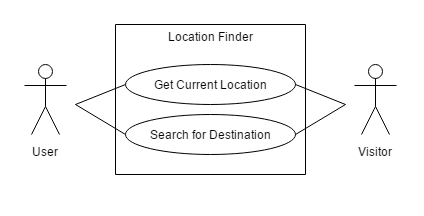
\includegraphics[scale=.7]{LocationFinder}
    \begin{flushleft}
    \textbf{Use case:} Get Current Location (R1.1)
    \newline
    	
    \textbf{Brief Description:}
    \newline
    The system shall determine the user's location or visitor's 		current location, whether indoors or outdoors.
    \newline
    
    \textbf{Initial Step-By-Step Description:}
    
    Before the use case can be initiated, the user has already logged in to the application. Visitors need not login but certain functionality will be restricted.
	\newline    
	
1. The user or visitor sends a request to get their current location.
    
2. The system obtains and returns the location of the user or visitor.
\end{flushleft}

\begin{flushleft}
    \textbf{Use case:} Search for Location (R1.2)
    \newline
    	
    \textbf{Brief Description:}
    \newline
    The system will allow users and visitors to search for any location based on their criteria.
    \newline
    
    \textbf{Initial Step-By-Step Description:}
    
    Before the use case can be initiated, the user or visitor has accessed search location menu option.
	\newline    
	
1. The user chooses to search the location by building name, lecture hall or venue name.

2. The system displays the choices to the user.

3. The user selects the desired location.

4. The system returns the location and gives user option to navigate to the location.
\end{flushleft}

\subsubsection{Navigation Module}
    Diagram:
    
    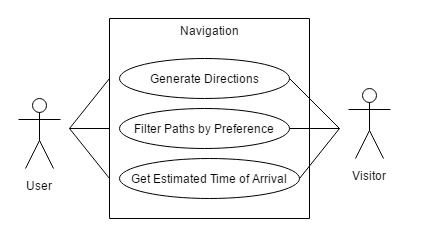
\includegraphics[scale=.7]{Navigation}
    
    \begin{flushleft}
    \textbf{Use case:} Get Directions of Location (R1.2)
    \newline
    	
    \textbf{Brief Description:}
    \newline
    The system shall navigate the user or visitor to their desired location.
    \newline
    
    \textbf{Initial Step-By-Step Description:}
    
    Before the use case can be initiated, the User has already logged into the application and has accessed the search location menu option. Visitors need not login but functionality will be restricted.
	\newline    
	
1. The user or visitor chooses to search the location by building name, lecture hall or venue name.

2. The system displays the choices to the user.

3. The user selects the desired venue. 

4. The system provides the directions of the location.

\end{flushleft}
    
    \begin{flushleft}
    \textbf{Use case:} Filter Directions by User Preference (R1.2)
    \newline
    	
    \textbf{Brief Description:}
    \newline
    The system shall filter the directions based on the user's or visitor's preferences.
    \newline
    
    \textbf{Initial Step-By-Step Description:}
    
    Before the use case can be initiated, the User has already logged into the application and has accessed the search location menu option. Visitors need not login but functionality will be restricted.
	\newline    
	
1. The user is prompted to select optional path filters.

2. The system updates the directions based on selected filters.


\end{flushleft}
    
    \begin{flushleft}
    \textbf{Use case:} Get Estimated Time of Arrival (ETA) (R1.2)
    \newline
    	
    \textbf{Brief Description:}
    \newline
    The system shall provide the user with an estimated time of arrival to the location they are navigating to.
    \newline
    
    \textbf{Initial Step-By-Step Description:}
    
    Before the use case can be initiated, the user or visitor has searched for a location to navigate to.
	\newline    
	
1. The user selects the venue to navigate to.

2. The system returns the optimal route and the ETA to the venue.

\end{flushleft}
   
   \subsubsection{Location Information Module}
    Diagram:
    
    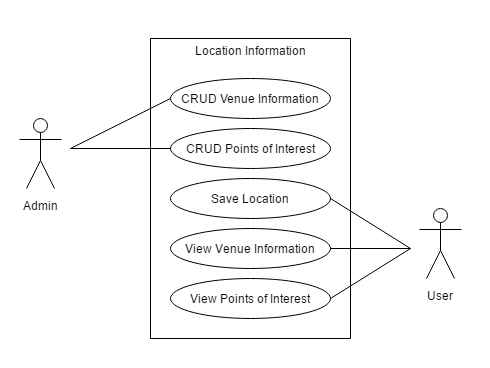
\includegraphics[scale=.7]{LocationInformation2} 
    
    \begin{flushleft}
    \textbf{Use case:} Save Location (R1.3)
    \newline
    	
    \textbf{Brief Description:}
    \newline
    The system shall allow the user to save a location.
    \newline
    
    \textbf{Initial Step-By-Step Description:}
    
    Before the use case can be initiated, the User has already searched for the desired location to save.
	\newline    
	
1.The user chooses to search for the location by building name, lecture hall or venue name or access previously searched venues.

2.The system displays the location to the user.

3.The user selects to save the location.

\end{flushleft}

\begin{flushleft}
    \textbf{Use case:} Create Read Update and Delete(CRUD) Venue Information (R2.1)
    \newline
    	
    \textbf{Brief Description:}
    \newline
    The system shall allow the different levels of users and agents the ability to create read update and delete information about different venues on campus.
    \newline
    
    \textbf{Initial Step-By-Step Description:}
    
    Before the use case can be initiated, the admin or user, depending on the case, has logged in to the application database. 
	\newline    
	
1. The user queries the database for the desired venue.

2. The system returns the results from the query.

3. The administrator selects from the results to perform a R.A.D operation.

4. The system updates the database after the changes have been made.

\end{flushleft}

\begin{flushleft}
    \textbf{Use case:} Create Read Update and Delete(CRUD) Points of Interest  (R2.1)
    \newline
    	
    \textbf{Brief Description:}
    \newline
    The system shall allow the admin the ability to create, read update and delete information about points of interest around campus based on their interests.
    \newline
    
    \textbf{Initial Step-By-Step Description:}
    
    Before the use case can be initiated, the admin or user, depending on the case, has logged in to the application database. 
	\newline    
	
1. The user selects from a list of points of interests.

2. The system returns points of interests based on the user's criteria.

3. The user selects which one they want to navigate to.

4. The system returns information about the venue and also directions to that venue.

\end{flushleft}

\begin{flushleft}
    \textbf{Use case:} View Information on locations  (R2.2)
    \newline
    	
    \textbf{Brief Description:}
    \newline
    The system shall allow the user to view information about locations, buildings and venues.
    \newline
    
    \textbf{Initial Step-By-Step Description:}
    
    Before the use case can be initiated, the user has searched for the desired location in order to obtain more information about the location.
	\newline    
	
1. The user chooses the location, venue or building.

2. The system returns information based on the user's criteria. 

3. The user access the desired information.

\end{flushleft}

\begin{flushleft}
    \textbf{Use case:} View Points of Interest  (R2.2)
    \newline
    	
    \textbf{Brief Description:}
    \newline
    The system shall allow the user to view information on points of interest.
    \newline
    
    \textbf{Initial Step-By-Step Description:}
    
    Before the use case can be initiated, the user has searched for the desired location in order to obtain more information about the location.
	\newline    
	
1. The user chooses the location, venue or building.

2. The system returns information based on the user's criteria. 

3. The user access the desired information.

\end{flushleft}

\subsubsection{Pedestrian Visualizer Module}
    Diagram:
    
    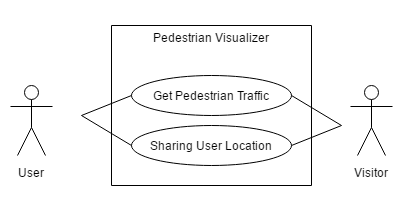
\includegraphics[scale=.7]{PedestrianVisualizer} 

\begin{flushleft}
    \textbf{Use case:} Get Pedestrian Traffic  (R1.2.1)
    \newline
    	
    \textbf{Brief Description:}
    \newline
    The system shall provide users with accurate information about pedestrian traffic based on how many devices are connected to certain WI-FI access points.
    \newline
    
    \textbf{Initial Step-By-Step Description:}
    
    Before the use case can be initiated, the user has searched for a location to navigate to.
	\newline    
	
1. The user has selected to navigate to a desired location.

2. The system returns general pedestrian traffic for the route selected and the optimal route with less pedestrian traffic.

\end{flushleft}

\begin{flushleft}
    \textbf{Use case:} Sharing Location  (R1.4)
    \newline
    	
    \textbf{Brief Description:}
    \newline
    The system shall allow users who have logged in to the application the ability to share their current location.
    \newline
    
    \textbf{Initial Step-By-Step Description:}
    
    Before the use case can be initiated, the user has obtained their current location.
	\newline    
	
1. The user selects to share their location with a friend or anyone with access to the application.

2. The systems generates a pin and allows the user to share their location.

\end{flushleft}

\subsubsection{Events and Activities Module}
    Diagram:
    
    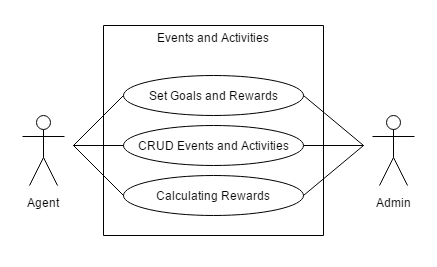
\includegraphics[scale=.7]{EventsAndActivities} 
    
\begin{flushleft}
    \textbf{Use case:} Calculating Rewards  
    \newline
    	
    \textbf{Brief Description:}
    \newline
    The system shall provide rewards for the user based on calculating the amount of steps the user has walked and also rewards based on class attendance and other activities such as that.
    \newline
    
    \textbf{Initial Step-By-Step Description:}
    
    Before the use case can be initiated, the user has logged into the application and selected an activity with a goal to meet.
	\newline    
	
1. The user selects an activity to take part in with a reward attached to it.

2. The system calculates if the requirements for the reward have been met such as the steps the user has taken and sums it up for the period within the goal. 

3. The user receives updates based on their rewards.

4. After completing the goal, the system provides the user with a reward.


\end{flushleft}

\begin{flushleft}
    \textbf{Use case:} Create Read Update and Delete(CRUD) Events and Activities  
    \newline
    	
    \textbf{Brief Description:}
    \newline
    The system shall allow the administrator or agent the ability to create, read, update or delete information on activities users might be interested in. 
    \newline
    
    \textbf{Initial Step-By-Step Description:}
    
    Before the use case can be initiated, the administrator or agent has logged in to the application database and has searched for a location to place an event or activity.
	\newline    

1. The administrator applies CRUD operations on the database for various activities.

2. The system updates the database after the changes have been.

\end{flushleft}

\begin{flushleft}
    \textbf{Use case:} Set goals and Rewards  
    \newline
    	
    \textbf{Brief Description:}
    \newline
    The system shall allow the administrator the ability to set and add goals and rewards for the users after inserting activity information. 
    \newline
    
    \textbf{Initial Step-By-Step Description:}
    
    Before the use case can be initiated, the administrator has logged in to the application database and activity other information has been inserted.
	\newline    

1. The administrator sets goals for users to match to in order to receive a reward.

2. The system tracks the user progress through the period the goal has been set.

3. The administrator reviews the progress report from the system and the appropriate reward is awarded to the user.


\end{flushleft}

\subsubsection{User Management Module}
    Diagram:
    
    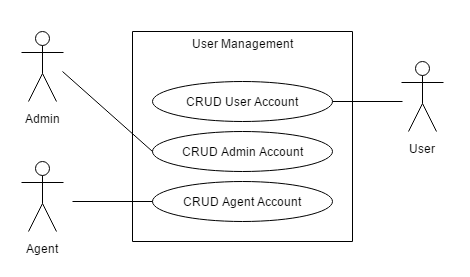
\includegraphics[scale=.7]{UserManagement} 
    
    \begin{flushleft}
    \textbf{Use case:} login  
    \newline
    	
    \textbf{Brief Description:}
    \newline
    The system shall provide the user, admin and agent with an interface to enter their credentials and login.
    \newline
    
    \textbf{Initial Step-By-Step Description:}
    
    There are no prerequisites for this action
	\newline    

1. The user, admin and agent inputs the required credentials.

2. The system validates the credentials and logs the user, admin or agent in if valid. 

\end{flushleft}

    \begin{flushleft}
    \textbf{Use case:} Create Read Update and Delete(CRUD) User Account  
    \newline
    	
    \textbf{Brief Description:}
    \newline
    The system shall provide the administrator, user and agent with the ability to CRUD their own accounts. 
    \newline
    
    \textbf{Initial Step-By-Step Description:}
    
    Before this use case can be initiated, the administrator, user and agent has logged in to the application database.
	\newline    

1. The user, admin or agent performs CRUD actions for their account.

2. The system changes the database based on the CRUD action.
 

\end{flushleft}
        
        \subsection{Actor-System Interaction Models}
			
			
        		\centering
					\textbf{UC1: Get Current Location}\\
       		 \small
       		 \begin{tabular}{|p{8cm}|p{8cm}|}
       		 \hline
       		 Preconditions: The user is logged on to the NavUP system.& \\
       		 \hline
       		 Actor: User & System: NavUP \\
        		\hline
       		  & 0.	The system displays the main menu options.\\
       		 \hline
       		 0.	TUCBW user chooses the "Current Location" menu option. & 2.	The system displays a Current Location menu.\\
        		\hline
       		3.	The user chooses the "Display my Location" option on the Current Location menu. & 4.	The system searches for (and displays) the user's current location.\\
        		\hline
       		5.	TUVEW the user views their current location. & \\
       		 \hline
        		Postconditions: None.& \\
        		\hline
        \end{tabular} 
     

			
        		\centering
					\textbf{UC2: Search for Location}\\
       		 \small
       		 \begin{tabular}{|p{8cm}|p{8cm}|}
       		 \hline
       		 Preconditions: The user is logged on to the NavUP system and has accessed the "Search Location" menu option.& \\
       		 \hline
       		 Actor: User & System: NavUP \\
        		\hline
       		 & 0.	The system displays three options whereby to search for a location.\\
       		 \hline
       		 1.	TUCBW user chooses to search the location by 

						a)	ETA.
						b)	Disability.
						c)	Pedestrian traffic.
 				& 2.	The system searches, TUCCW Search for Location, for (and displays) the location choices to the user based on the option (a-c) chosen.\\
        		\hline
       		 3.	The user selects the desired location. & 4.	The system\\ returns the location and gives user option to navigate to the location.\\
        		\hline
       		 5.	TUCEW user chooses to navigate to desired location. & \\
       		 \hline
        		Postconditions: The system loads directions from the database.& \\
        		\hline
        \end{tabular} 

		
        		\centering
					\textbf{UC3: Get Directions of Location}\\
       		 \small
       		 \begin{tabular}{|p{8cm}|p{8cm}|}
       		 \hline
       		 Preconditions: The user is logged on to the NavUP system and has accessed the "Search Location" menu option.& \\
       		 \hline
       		 Actor: User & System: NavUP \\
        		\hline
       		 & 0.	The system displays three options whereby to search for a location.\\
       		 \hline
       		 1.	TUCBW user chooses to search the location by 

						\\a)	ETA.
						\\b)	Disability.
						\\c)	Pedestrian traffic.
 & 2.	The system searches, TUCCW Search for Location, for (and displays) the location choices to the user based on the option (a-c) chosen. \\
        		\hline
       		 3.	The user selects the desired location. & 4.	The system presents optimal routes to the location. \\
        		\hline
       		 5.	The user chooses the route to follow. & 6.	The system provides the directions to the location (and asks the user if they want to save the location, TUCCW Save Location).\\
        		\hline
        		7.	TUCEW user following the directions to the desired location. & \\
       		 \hline
        		Postconditions: None.& \\
        		\hline
        \end{tabular} 
        

		
        		\centering
					\textbf{UC4: Filter Directions by User Preference}\\
       		 \small
       		 \begin{tabular}{|p{8cm}|p{8cm}|}
       		 \hline
       		 Preconditions: The User has already logged into the application and has accessed the search location menu option. Visitors need not login but\\ functionality will be restricted.& \\
       		 \hline
       		 Actor: User & System: NavUP \\
        		\hline
       		 & 0.	The system displays options whereby to search for a location.\\
       		 \hline
       		 1.	TUCBW user chooses to search the location by \\

						\\a)	ETA.
						\\b)	Disability.
						\\c)	Pedestrian traffic.
 				& 2.	The system updates the directions based on:\\

						\\a)	The fastest route.
						\\b)	A route suitable for users with a disability.
						\\c)	A route with minimal of maximal pedestrian traffic.
\\
        		\hline
       		 	3.	TUCEW the user to navigating to desired location. &\\
       		 \hline
        		Postconditions: None.& \\
        		\hline
        \end{tabular} 
     

		
        		\centering
					\textbf{UC5: Get Estimated Time of Arrival (ETA)}\\
       		 \small
       		 \begin{tabular}{|p{8cm}|p{8cm}|}
       		 \hline
       		 Preconditions: The user has searched for a location to navigate to.& \\
       		 \hline
       		 Actor: User & System: NavUP \\
        		\hline
       		  & 0.	The system searches, TUCCW Search for Location, for (and displays) the location choices to the user based on the option chosen.\\
       		 \hline
       		 1.	The user selects the desired location. & 2.	The system calculates general and optimal routes, TUCCW Get Pedestrian Traffic.\\
        		\hline
       		 3.	The user chooses a route. & 4.	The system calculates the ETA to the desired venue (and displays directions to the desired location).\\
        		\hline
       		 5.	TUCEW user views and follows the directions. & \\
       		 \hline
        		Postconditions: None.& \\
        		\hline
        \end{tabular} 
        

		
        		\centering
					\textbf{UC6: Save Location}\\
       		 \small
       		 \begin{tabular}{|p{8cm}|p{8cm}|}
       		 \hline
       		 Preconditions:Before the use case can be initiated, the User has already searched for the desired location to save.& \\
       		 \hline
       		 Actor: User & System: NavUP \\
        		\hline
       		 & 0.	The system provides the directions to the location (and asks the user if they want to save the location, TUCCW Save Location).\\
       		 \hline
       		 1.	TUCBW user choosing to:

						a)	Save the location.
						b)	Not save the location.
 				& 2.	The system (updates the database and) starts shows directions \\to the location.

\\a) Updates the database by adding the location.
\\b) Leaves the database as is.
\\
        		\hline
       		 3.	TUCEW user following the directions to the desired location. &\\
       		 \hline
        		Postconditions: The system database is altered. \\
        		\hline
        \end{tabular} 
       

		
        		\centering
					\textbf{UC7: Create Read Update and Delete(CRUD) Venue Information}\\
       		 \small
       		 \begin{tabular}{|p{8cm}|p{8cm}|}
       		 \hline
       		 Preconditions: The admin or user, depending on the case, has logged in to the application database.& \\
       		 \hline
       		 Actor: User & System: NavUP \\
        		\hline
       		 & 0.	The system shows different venues.\\
       		 \hline
       		 1.	TUCBWThe user queries the database for the desired venue.\\
 				&2.	The system returns the results from the query.\\
        		\hline
       		 3.	The administrator selects from the results to perform a R.A.D operation. & 4.	The system updates the database after the changes have been made.\\
				\hline
					5.	TUCEW user views the different venues.&\\
       		 \hline
        		Postconditions: The system database is altered. \\
        		\hline
        \end{tabular} 
       

				
        		\centering
					\textbf{UC8: Create Read Update and Delete(CRUD) Venue Information}\\
       		 \small
       		 \begin{tabular}{|p{8cm}|p{8cm}|}
       		 \hline
       		 Preconditions: The admin or user, depending on the case, has logged in to the application database.& \\
       		 \hline
       		 Actor: User & System: NavUP \\
        		\hline
       		 & 0.	The system shows different points of interest.\\
       		 \hline
       		4.	TUCBW administrator/user decides to:\\

\\e)	Create a point of interest.
\\f)	Read a point of interest.
\\g)	Update a point of interest.
\\1.	Delete a point of interest.

 				&2.	2.	The system:\\

\\a)	Updates a point of interest (by inserting the event/activity into the \\database).
\\b)	Fetches a point of interest from the database for viewing.
\\c)	Updates information in the database about a point of interest.
\\d)	Deletes an point of interest from the database.
\\
        		\hline
       		 	3.	TUCEW the administrator/user viewing changes to events/activities. &\\
       		 \hline
        		Postconditions: The system database is altered. \\
        		\hline
        \end{tabular} 
       
		
        		\centering
					\textbf{UC9: View Information on Locations}\\
       		 \small
       		 \begin{tabular}{|p{8cm}|p{8cm}|}
       		 \hline
       		 Preconditions: The user has searched for the desired location to obtain more information about the location.& \\
       		 \hline
       		 Actor: User & System: NavUP \\
        		\hline
       		& 0.	The system searches for a location, TUCCW Search Location.\\
       		 \hline
       		 1.	TUCBW user choosing to view more information about a location.\\  & 2.	The system fetches the necessary information from the database, and display it.\\
        		\hline
       		 3.	TUCEW user viewing information on locations. &\\
       		 \hline
        		Postconditions: None. & \\
        		\hline
        \end{tabular} 
      

		
        		\centering
					\textbf{UC10: View Points of Interest}\\
       		 \small
       		 \begin{tabular}{|p{8cm}|p{8cm}|}
       		 \hline
       		 Preconditions: The user has provided the application with information about their interests.& \\
       		 \hline
       		 Actor: User & System: NavUP \\
        		\hline
       		 & 0.	The system displays a list of points of interests based on the user's criteria.\\
       		 \hline
       		 1.	TUCBW user selects a point of interest. & 2.	The system (fetches information from the database and) displays information about that venue (and displays directions to that venue).\\
        		\hline
       		 3.	TUCEW user views the information and directions. &\\
       		 \hline
        		Postconditions: None.& \\
        		\hline
        \end{tabular} 
      

		
        		\centering
					\textbf{UC11: Get Pedestrian Traffic}\\
       		 \small
       		 \begin{tabular}{|p{8cm}|p{8cm}|}
       		 \hline
       		 Preconditions: The user has searched for a location to navigate to.& \\
       		 \hline
       		 Actor: User & System: NavUP \\
        		\hline
       		  & 0.	The system searches, TUCCW Search for Location, for (and displays) the location choices to the user based on the option chosen.\\
       		 \hline
       		 1.	The user selects the desired location. & 2.	The system returns general pedestrian traffic for the selected route, and an optimal route with less pedestrian traffic.\\
        		\hline
       		 3.	The user chooses a route. & 4.	The system displaysdirections following the chosen route to the desired location.\\
        		\hline
       		 5.	The user chooses:\\

						\\a)	General route.
					\\	b)	Optimal route.
			 & 6.	The system displays directions for:\\

					\\a)	The general route to the user's desired location.
					\\b)	The optimal route to the user's desired location.
 \\
        		\hline
        		7.	The user views and follows the directions to their desired location. & \\
       		 \hline
        		Postconditions: None.& \\
        		\hline
        \end{tabular} 
     

		
        		\centering
					\textbf{UC12: Sharing Location}\\
       		 \small
       		 \begin{tabular}{|p{8cm}|p{8cm}|}
       		 \hline
       		 Preconditions: The user has obtained their current location.& \\
       		 \hline
       		 Actor: User & System: NavUP \\
        		\hline
       		  & 0.	The system displays the user's current location, TUCCW Get Current Location.\\
       		 \hline
       		 1.	TUCBW user selects to share their location with anyone who has access to the application. & 2.	The system generates a pin and allows the user to share their location (and displays a confirmation message).\\
        		\hline
       		3.	TUCEW user acknowledging the confirmation message. &\\
       		 \hline
        		Postconditions: None.& \\
        		\hline
        \end{tabular} 
       

		

	
        		\centering
					\textbf{UC13: Calculating Rewards}\\
       		 \small
       		 \begin{tabular}{|p{8cm}|p{8cm}|}
       		 \hline
       		 Preconditions: The user has logged into the application and selected a goal to meet.& \\
       		 \hline
       		 Actor: User & System: NavUP \\
        		\hline
       		 & 0.	The system shows directions to the desired location.\\
       		 \hline
       		 1.	The user views and follows the directions provided. & 2.	The system calculates the steps the user takes (and updates the database).\\
        		\hline
       		 3.	The user keeps walking until a goal is met. & 4.	The system sums up steps for a period, and sends updates to the user.\\
        		\hline
       		 5.	The user receives updates. & 6.	The system determines if goals are met, and notifies the user of rewards (and updates the system database).\\
        		\hline
        		7.	The user views their rewards for goals met. & \\
       		 \hline
        		Postconditions: The system database is altered. & \\
        		\hline
        \end{tabular} 
     

		
        		\centering
					\textbf{UC14: Create Read Update and Delete(CRUD) Events and Activities}\\
       		 \small
       		 \begin{tabular}{|p{8cm}|p{8cm}|}
       		 \hline
       		 Preconditions: The administrator or agent has logged in to the application database and has searched for a location to place an event or activity.& \\
       		 \hline
       		 Actor: User & System: NavUP \\
        		\hline
       		 & 0.	The system shows different venues.\\
       		 \hline
       		1.	TUCBW administrator decides to:\\

\\a)	Create an event/activity.
\\b)	Read an event/activity.
\\c)	Update an event/activity.
\\d)	Delete an event/activity.
 &2.	The system:

\\a)	Updates an event/activity (by inserting the event/activity into the \\database).
\\b)	Fetches an event/activity from the database for viewing.
\\c)	Updates information in the database about an event/activity.
\\d)	Deletes an event/activity from the database.
\\
        		\hline
       		3.	TUCEW the administrator viewing changes to events/activities.&\\
       		 \hline
        		Postconditions: The system database is altered. & \\
        		\hline
        \end{tabular} 
   


        		\centering
					\textbf{UC15:Set goals and Rewards}\\
       		 \small
       		 \begin{tabular}{|p{8cm}|p{8cm}|}
       		 \hline
       		 Preconditions: The administrator has logged in to the application database and activity other information has been inserted.& \\
       		 \hline
       		 Actor: User & System: NavUP \\
        		\hline
       		 &0.	The system shows a rewards interface.\\
       		 \hline
       		1.	TUCBW administrator sets goals for users to match to in order to receive a reward.
 &2.	The system adds the goal to the database , and tracks the user progress through the period the goal has been set, TUCCW Calculating Rewards.
\\
        		\hline
       		3.	TUCEW administrator reviews the progress report from the system and the appropriate reward is awarded to the user.&\\
       		 \hline
        		Postconditions: The system database is altered. & \\
        		\hline
        \end{tabular} 
      

		
        		\centering
					\textbf{UC16: Login}\\
       		 \small
       		 \begin{tabular}{|p{8cm}|p{8cm}|}
       		 \hline
       		 Preconditions: None.& \\
       		 \hline
       		 Actor: User & System: NavUP \\
        		\hline
       		 &0.	The system shows a login interface.\\
       		 \hline
       		1.	TUCBW user, admin and agent inputs the required credentials.\\
 &2.	The system validates the credentials (by fetching the necessary information from the system database),and logs the user, admin or agent in if valid.
\\
        		\hline
       		3.	TUCEW user, admin and agent logs in and view the main menu.&\\
       		 \hline
        		Postconditions: The system is notified that a user, admin or agent has logged in. & \\
        		\hline
        \end{tabular} 
        
	
        		\centering
					\textbf{UC17: Create Read Update and Delete(CRUD) User Account}\\
       		 \small
       		 \begin{tabular}{|p{8cm}|p{8cm}|}
       		 \hline
       		 Preconditions: The administrator, user and agent has logged in to the application database.& \\
       		 \hline
       		 Actor: User & System: NavUP \\
        		\hline
       		 &0.	The system shows a profile interface.\\
       		 \hline
       		1.	TUCBW the user, admin or agent performing CRUD actions for their account such as:\\

\\a)	Read.
\\b)	Update.
\\c)	Delete.
 & 2.	The system changes the database based on the CRUD action:

\\a)	The system fetches the user information form the database for viewing.
\\b)	The system updates the user information in the database.
\\c)	The system deletes the user from the system database and logs them out.

\\
        		\hline
       		3.	TUCEW user, admin and agent:

\\a)	Viewing their profile.
\\b)	Gets logged out.
&\\
       		 \hline
        		Postconditions: The administrator, user of agent is logged out or deleted from the system, and the system database is altered. & \\
        		\hline
        \end{tabular} 
    	\subsection{Traceability Matrix}
        \begin{table}[h!]
        \centering
        \small
        \begin{tabular}{|c|c|c|c|c|c|}
        \hline
        Requirements & Navigation & Heat Maps & Saved and Current Locations & Push Notifications & Activities \\
        \hline
        R1 & & & & &\\
        \hline
        R1.1 & & & X & &\\
        \hline
        R1.2 & & & & &\\
        \hline
        R1.2.1 & & X & & &\\
        \hline
        R1.3 & & & X & & \\
        \hline
        R1.4 & X & & & & \\
        \hline
        R2 & & & & & \\
        \hline
        R2.1 & & & & X & \\
        \hline
        R2.2 & & & X & & \\
        \hline
        R2.3 & & & X & & \\
        \hline
        R2.4 & X & & & & \\
        \hline
        R3 & & & & & \\
        \hline
        R3.1 & & & & & \\
        \hline
        R3.1.1 & & & & X & \\
        \hline
        R4 & & & & & X \\
        \hline
        \end{tabular}
        
        \end{table}
    \subsection{Performance Requirements}
    \subsection{Design Constraints}
    \subsection{System Software Attributes}
    \subsection{Other Requirements}
    
\section*{Appendixes}
\section*{Index}
\end{document}
